\documentclass[Softwaredesign/Softwaredesign_main.tex]{subfiles}
\begin{document}

\section{CupSensor\_IF}
Der skal udvikles en CupSensor\_IF klasse på PlayerSideApp som har til opgave at håndtere input/output for alle 6 Cup Sensors på en player side. Dette er udvilket på baggrund af hardwaren beskrevet i \ref{hwdesign:sec:CupSensor}. Som opsummering benyttes der en multiplexer som styre hvilken cup sensor som der sættes til blinke med dens IR LED. Herefter bruges der udtrykket der styres hvilke 'sensor der læses'. Multiplexeren styres af et register Control\_Reg\_Led. Inputtet ender med at blive læst med en Delta Sigma ADC, med et differentiabelt input. Til forventede signaler er der kun positive signaler. Der benyttes sinc4 filteret i ADC'en. Dette betyder at udgangen først er korrekt efter 4 samples hvis der sker et step i indgangssignalet. Til at læse signalet fra ADC'en benyttes en DMA (Direct memory access) komponent som genererer et interrupt når den er færdig.

Der er til software design af CupLight\_IF, udviklet et klassediagram. Diagrammet kan ses på figur \ref{fig:CupSensor-IF-classDiagram}. Det vil være uhensigtsmæssigt at lave alt i en klasse. Klassen CupSensor\_IF er den klasse som GameController interagere med. De resterende klasser er en del af en custom component i PSoC se afsnit.  CupSensor er hoved-klassen for CupSensor blokken. Den skal som alle andre PSoC komponenter startes vha. Start metoden. Denne metode sørge for at starte og opsætte de forskellige hardware komponenter og interrupts. Derudover skal de 6 instanser for CupSensorUnit initieres. Som en del af denne metode skal DMA'en opsættes. Koden til dette genereres vha. PSoC Creators DMA Wizard. Da man som tidligere beskrevet skal vente 4 samples efter et step på indgangen, opsættes DMA'en til kun at generere et interrupt efter hver 6. sample. Det er 6 frem for 4 Da andre dele af systemet også vil tage noget tid at reagere på et step. Det step der tales om, er ændringen i hvilken sensor der sættes til at blinke. Da to sensorer ikke nødvendigvis har samme output, vil ændringen opfattes som et step. ADC'en har en samplerate på 2500 sps, når kun hver 6. måling er brugbar svare det til en samplerate på ca. 417 sps. Men da der skal læses fra 6 Cup Sensors, er sampleraten for en given sensor kun ca 70 sps. Dette vil betyde at at den maksimale frekvens der kan måles er 35Hz, eller signaler med en periode på ca 29 ms eller længere. Det signal der for sensoren skal analyseres som har den højeste frekvens er når en bold rammer i. Dette har en periode på ca 200ms. Derfor er dette en god nok løsning.

Der skal i CupSensor klassen være get metoderne til CupStatus og HitStatus. Det er metoderne getStatus() og getHitStatus(). Der er det to funktioner statusCallback og hitStatusCallback som har funktionspointere som argumenter. Disse funktioner bruges til at indstille hvilken metode der skal kaldes når cupStatus eller hitStatus ændres. Disse metoder kaldes af CupSensor\_IF klassen som sørger for at de to funktioner der kaldes er updateCupStatus og updateHitStatus i GameController klassen (i PlayerSideApp).
Som tidligere beskrevet sker der et interrupt når der er en ny måling fra ADC'en (kun hver 6. måling). Til dette interrupt er der en ISR kaldes CY\_ISR(newValueInterruptHandler). Indholdet af denne interrupt handler kan ses på figur \ref{fig:CupSensor-IF-getting-reading}. 
 
\begin{figure}[H]
    \centering
    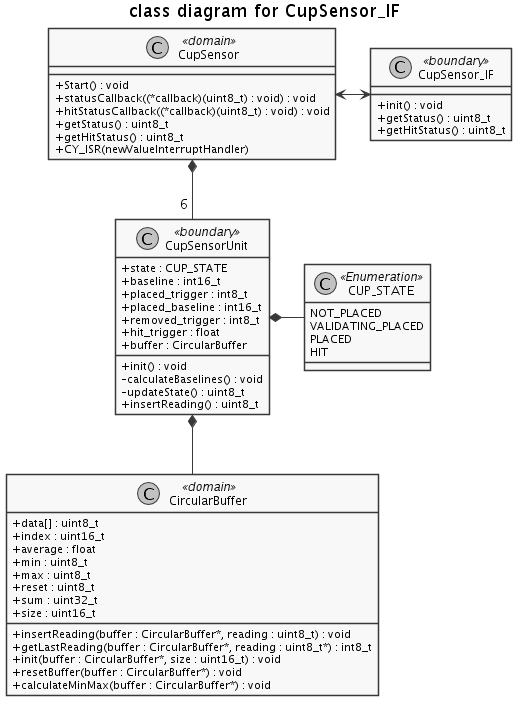
\includegraphics[width=0.8\textwidth]{Softwaredesign/CupSensor_IF/graphics/classDiagram.png}
    \caption{.}
    \label{fig:CupSensor-IF-classDiagram}
\end{figure}

Der er 6 objekter af klassen CupSensorUnit. Denne repræsentere hver Cup Sensor. Hver CupSensorUnit har en CUP\_STATE til at holde styr på tilstanden af den givne Cup Sensor. Derudover er der en CircularBuffer klasse som bruges til at lagre de seneste målinger for hver CupSensorUnit.

Der kan ses på sekvensdiagrammet på figur \ref{fig:CupSensor-IF-getting-reading} hvad der sker når der modtages en ny måling fra ADC'en. Det første der sker er at ændre på hvilken sensor der læses. Dette gøres ved at ændre på Control\_Reg\_Led registeret. Denne komponent har sin egen 'klasse' hvor Read funktionen bruges til at læse hvad den nuværende tilstand værdi er. Herefter opdateres dens værdi ved at tælle en op. Der sørges for at Control\_Reg\_Led kun vil nå op til 5, hvorefter den skifter til 0. 
Efter dette kaldes insertReading metoden i den CupSensorUnit som læsningen stammer fra, bestemt af værdien af Control\_Reg\_Led. Denne metode indsætter værdien i dens buffer, som er en CicularBuffer. Herefter kaldes updateState som på baggrund af den nye værdi og de beregnede 'baselines' (beskrives senere), opdatere tilstanden i tilstandsmaskinen (beskrives senere).  

buffer bruges hovedsagligt til at beregne et gennemsnit, da det skal bruges til at beregne 'baselines' som skal beregnes når calculateBaselines kaldes. Denne funktion beregner ud fra gennemsnittet af 
Denne metode returnerer om tilstanden ændres, hvis den gør kaldes de nødvendige metoder i GameController. 
\begin{figure}[H]
    \centering
    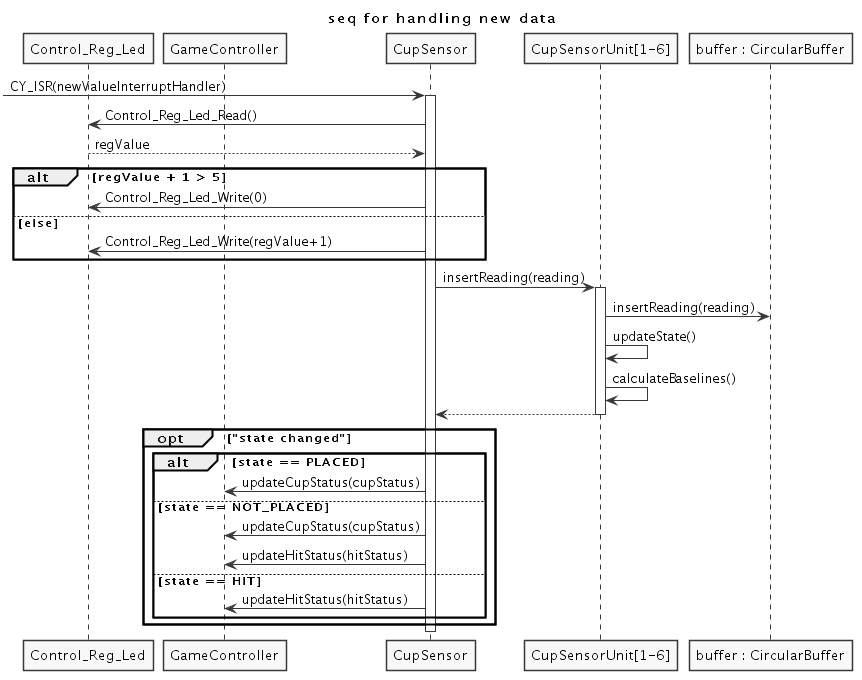
\includegraphics[width=1\textwidth]{Softwaredesign/CupSensor_IF/graphics/getting_reading.png}
    \caption{.}
    \label{fig:CupSensor-IF-getting-reading}
\end{figure}

Til at styre tilstanden for CupSensorUnit udvikles en tilstandsmaskine som ses på figur \ref{fig:CupSensor-IF-state}. Der er af åbenlyse grunde de tre tilstande NOT\_PLACE, PLACED og HIT. Men der er også en tilstand VALIDATING\_PLACED. Denne tilstand er til for at minimere risikoen for at der sker en falsk transition til tilstanden PLACED, da det kræver at signalet skal være højt i en længere tid, 20 samples eller ca. 300ms. Dette vil gøre systemet langsommere, men mere pålideligt. Som det ses på figur \ref{fig:CupSensor-IF-state}, benyttes der det der kaldes 'baseline', som er inspiration fra CapSense, som blev undersøgt i teknologiundersøgelsen. Der der benævnes 'reading', er den målte værdi minus den beregnede 'baseline'. Til at skifte mellem de forskellige tilstande benyttes der forskellige grænseværdier som reading skal være over/under. Til at skifte til tilstanden VALIDATING\_PLACED og tilbage til NOT\_PLACED, både fra VALIDATING\_PLACED, PLACED og HIT, benyttes der absolutte grænseværdier, placed\_trigger og removed\_trigger. Men til at skifte til HIT benyttes der en grænseværdi, hit\_trigger, der er relativ til værdien, placed\_baseline, når der er placeret en kop. Dette er til for at der fx. for en kop med meget øl, og derfor lille placed\_baseline, skal en mindre absolut ændring til for at detektere at en bold rammer i. Der vil komme en mindre ændring da bolden vil være længere væk fra sensoren.

\begin{figure}[H]
    \centering
    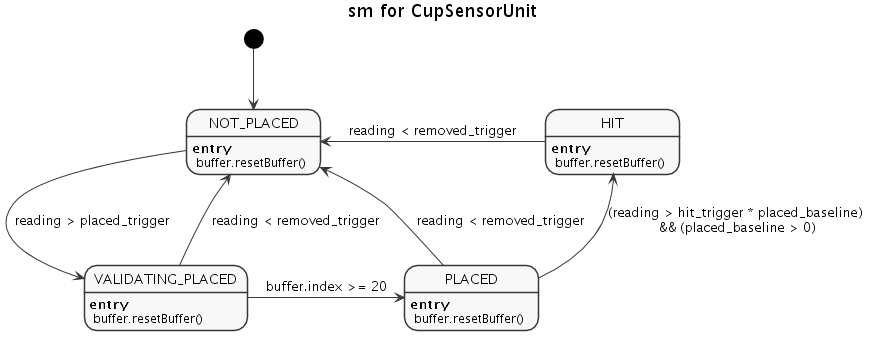
\includegraphics[width=1\textwidth]{Softwaredesign/CupSensor_IF/graphics/state.png}
    \caption{.}
    \label{fig:CupSensor-IF-state}
\end{figure}

Til at bestemme de forskellige grænseværdier der udført nogle målinger, hvor der placeres/fjernes en kop flere gange, og der tabes en bold flere gange. Dette udføres med forskellige mængder øl, den øvre og nedre grænse for mængden af øl beskrevet i kravene samt den nominelle værdi, 110ml. Det er forsøgt at bestemme grænseværdierne vha. konfidensniveau beregninger, i det der antages at målingerne er normalfordelte. Målingerne blev udført på et tidspunkt hvor der ikke var kendskab til denne type beregningerne, og det kan diskuteres om det er en realistisk antagelse at målingerne er normalfordelte. Derfor blev der hovedsageligt benyttet de maksimale og minimale målinger til at bestemme grænseværdierne.  



\subsection{Valg af kalibreringskoefficienter}
For at bestemme placed_trigger måles den aflæste den signalet fra sensoren 10 gange når der står en kop med 90ml, og 10 gange med 110ml og 10 gange med 130ml.
Det mindste signal kom fra den med 130ml.
Der er middelværdien 21 relativ til baseline, med en præcision med 95\% konfidensniveau på 12. Den målte værdi kan dermed risikere at være 9 relativ til baseline. Men idet koppen placeres er signalet højere. Der måles derfor hvor stor dette signal bliver, 10 gange for hver mængde øl (90ml, 110ml og 130ml). For både 90ml og 110ml er der en stor varians, men da de begge har et højt signal når der er en kop, bruges disse målinger ikke. For 130ml er der en middelværdi på 33 relativ til baseline, og en præcision på 22 (med 95\% konfidensniveau). Det vil sige at det kan risikeres at det laveste signal er 33-22=11 relativ til baseline. Derfor sættes placed_trigger til 11. 

removed_trigger sættes lidt under den laveste mulige stationære værdi der kan måles (med et konfidensniveau på 95\%). Denne er som tidligere beskrevet, 9 relativ til baseline. Derfor sættes removed_trigger til 8.

For at bestemme hit_trigger tabes en bold ned i en kop som står på sensoren 10 gange for hver mængde øl (90ml, 110ml, 130ml). Der måles den maksimale signal fra sensoren idet bolden rammer i, hver gang. Det antages først at dette er normalfordelt. Der er så stor en standardafvigelse at peaksignalet med et konfidensniveau på 95\% kan risikere at være under baseline signalet. Dette giver ikke nogen mening, og er ikke brugbar. Det vil måske være mulgit at bruge normalfordeling til at beregne hit_trigger, hvis der foretages flere målinger. Men det er ikke muligt med de målinger der er blevet foretaget. Derfor vælges der så lav en hit_trigger som muligt uden at signalet kommer op over hit_trigger idet koppen fjernes. Igen er dataen ikke ret brugbar til at benytte beregninger ud fra normalfordellinger. Men det observeres at det maksimale signal der fremkommer ved at fjerne koppen er 1.79 gange signalet for når der står en kop med øl (i forhold til baseline).
Derfor vælges en lidt større værdi end denne. hit_trigger sættes til at være 1.9. Dette er ikke den ideele måde at bestemme hit_trigger på, men det er det er testet og 1.9 er en god værdi til at detektere så mange bolde der ramme i som muligt samtidig med at der ikke detekteres.

\end{document}